\NoBgThispage
\chapter{MapAlign: Training and Model Approaches}

This chapter provides a detailed examination of the developed architecture throughout its various phases, focusing particularly on the two approaches that yielded the most promising results.

\section{First Approach}

The initial approach involved designing a model to perform the task described in previous chapters without reconstructing a complete Bird's-Eye View (BEV) from the camera images. Rather than using raw images, the model directly worked with features extracted from them, focusing on the pre-existing obstacle reconstructions.

In this approach, the network aimed to estimate the translation along the three spatial axes (\( x, y, z \)) and the heading angle in radians.

This model, named PoseNet, processes data using input from the loader described earlier. All inputs are combined to create an 11-channel tensor optimized for pose estimation tasks. PoseNet has several key components: a preprocessor, a backbone, a decoder, and output layers. 

The **BEVPreprocessor** prepares the input data with a simple structure consisting of a single convolutional layer with just 0.0013 million parameters, keeping it efficient. The **Backbone**, based on the BiSeNetV1 architecture \cite{DBLP:journals/corr/abs-1808-00897}, is the most complex component, with 12.63 million parameters. The backbone uses two paths: 

- **Spatial Path**: Designed with a small stride to preserve spatial details, this path captures high-resolution features through several convolutional layers, emphasizing fine-grained spatial information.
- **Context Path**: This path quickly down-samples the input to expand the receptive field, helping the model capture broader context. It utilizes Attention Refinement Modules (ARMs) and additional convolutional layers. ARMs allow the model to focus on important regions within the image, significantly contributing to the model's parameter count.

A **Feature Fusion Module** is used to efficiently combine the features from the Spatial and Context Paths.

The **Decoder** then upsamples these features to restore them to the original input resolution, with a parameter count of 0.0924 million. The role of the decoder is to convert high-level, low-resolution features back into the detailed, high-resolution format needed for accurate output. This component ensures that the model’s outputs match the input image's scale, making the model suitable for precise localization tasks.

The head, called **PoseSegHead**, generates the segmentation output, while a fully connected (Fc) layer finalizes the pose estimation. This design enables efficient and accurate pose analysis. The model’s total parameter count is optimized to balance processing efficiency and accuracy.

Figure \ref{fig:enter-label} illustrates the complete model structure.

\begin{figure}
    \centering
    \includegraphics[width=0.75\linewidth]{LateX//figs/modello_POSENET.pdf}
    \caption{Structure of the PoseNet Model}
    \label{fig:enter-label}
\end{figure}

The primary goal was to accurately predict the four values: translations along the \( x, y, z \) axes and the heading angle. Alongside model design, appropriate loss functions were also defined. As described in Chapter 1, the three loss functions used were L1, L1-smooth, and MSE.

The main loss function encompassed all four parameters, with two additional specialized losses for the translation and heading angle. The heading angle was especially critical and challenging to learn accurately, so this structure was consistent across different model versions.

The initial iterations used the following high-level parameters:

- **Data augmentation** included body rotations between -30° and 30° and horizontal and vertical shifts up to 10%.
- **Optimizer**: Training used the SGD optimizer with a base learning rate of 0.1 and a batch size of 64.
- **Learning Rate Scheduler**: The scheduler was WarmupPolyLR with a warm-up period of 5,000 iterations, capped at a maximum of 100,000 iterations.
- **Automatic Mixed Precision (AMP)** was enabled to improve training speed and resource use.

The learning rate demonstrated the following behavior during training:

\begin{figure}[H]
    \centering
    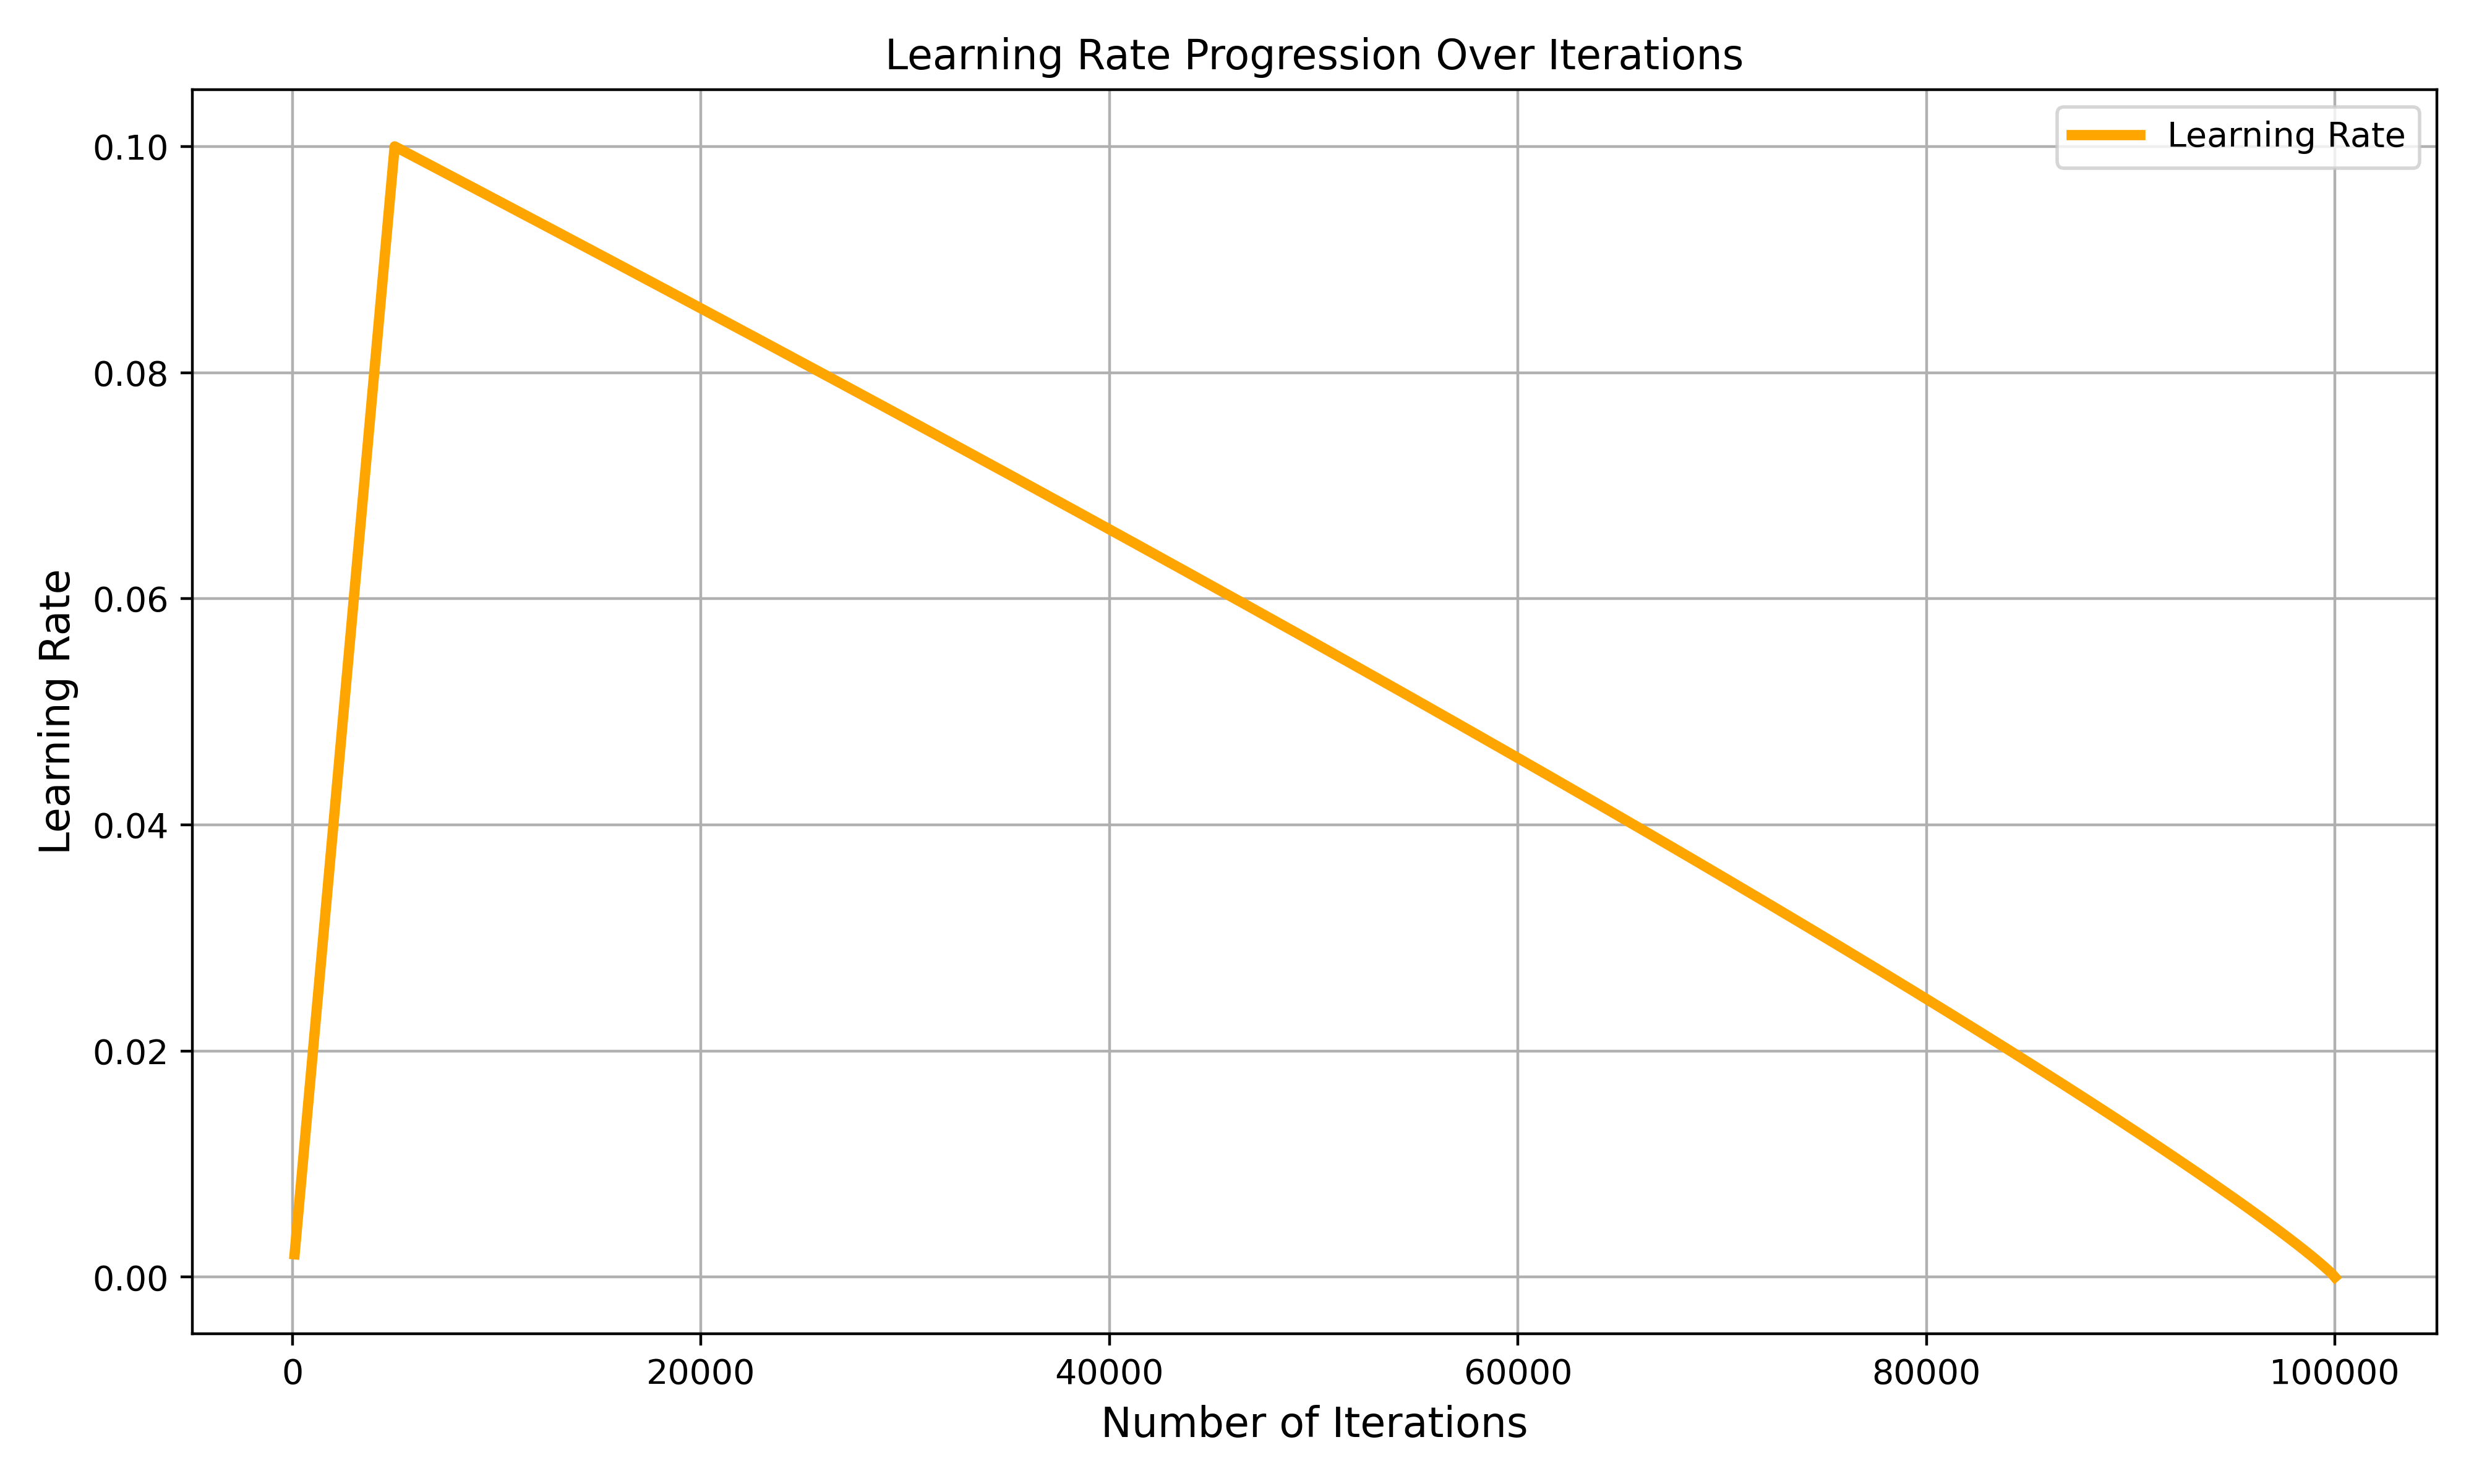
\includegraphics[width=0.75\linewidth]{LateX//figs/learning_rate_progression.png}
    \caption{Learning Rate Progression During Training}
    \label{fig:learning-rate-progression}
\end{figure}

Checkpoints were saved every 100 iterations, and evaluations were conducted every 5,000 iterations using the PoseEvaluator. The evaluator calculated an L1 loss on a validation set to objectively assess the model’s performance.

Training was accelerated with CUDA, using CuDNN benchmarking for improved speed. Initial training sessions utilized only a portion of the dataset to refine the model’s structure and functionality before scaling to the full dataset.

\subsubsection*{MSE}
The first training session used MSE as the loss function, along with the parameters described above. This approach resulted in a steadily decreasing loss, as shown in the figure below:

\begin{figure}[H]
    \centering
    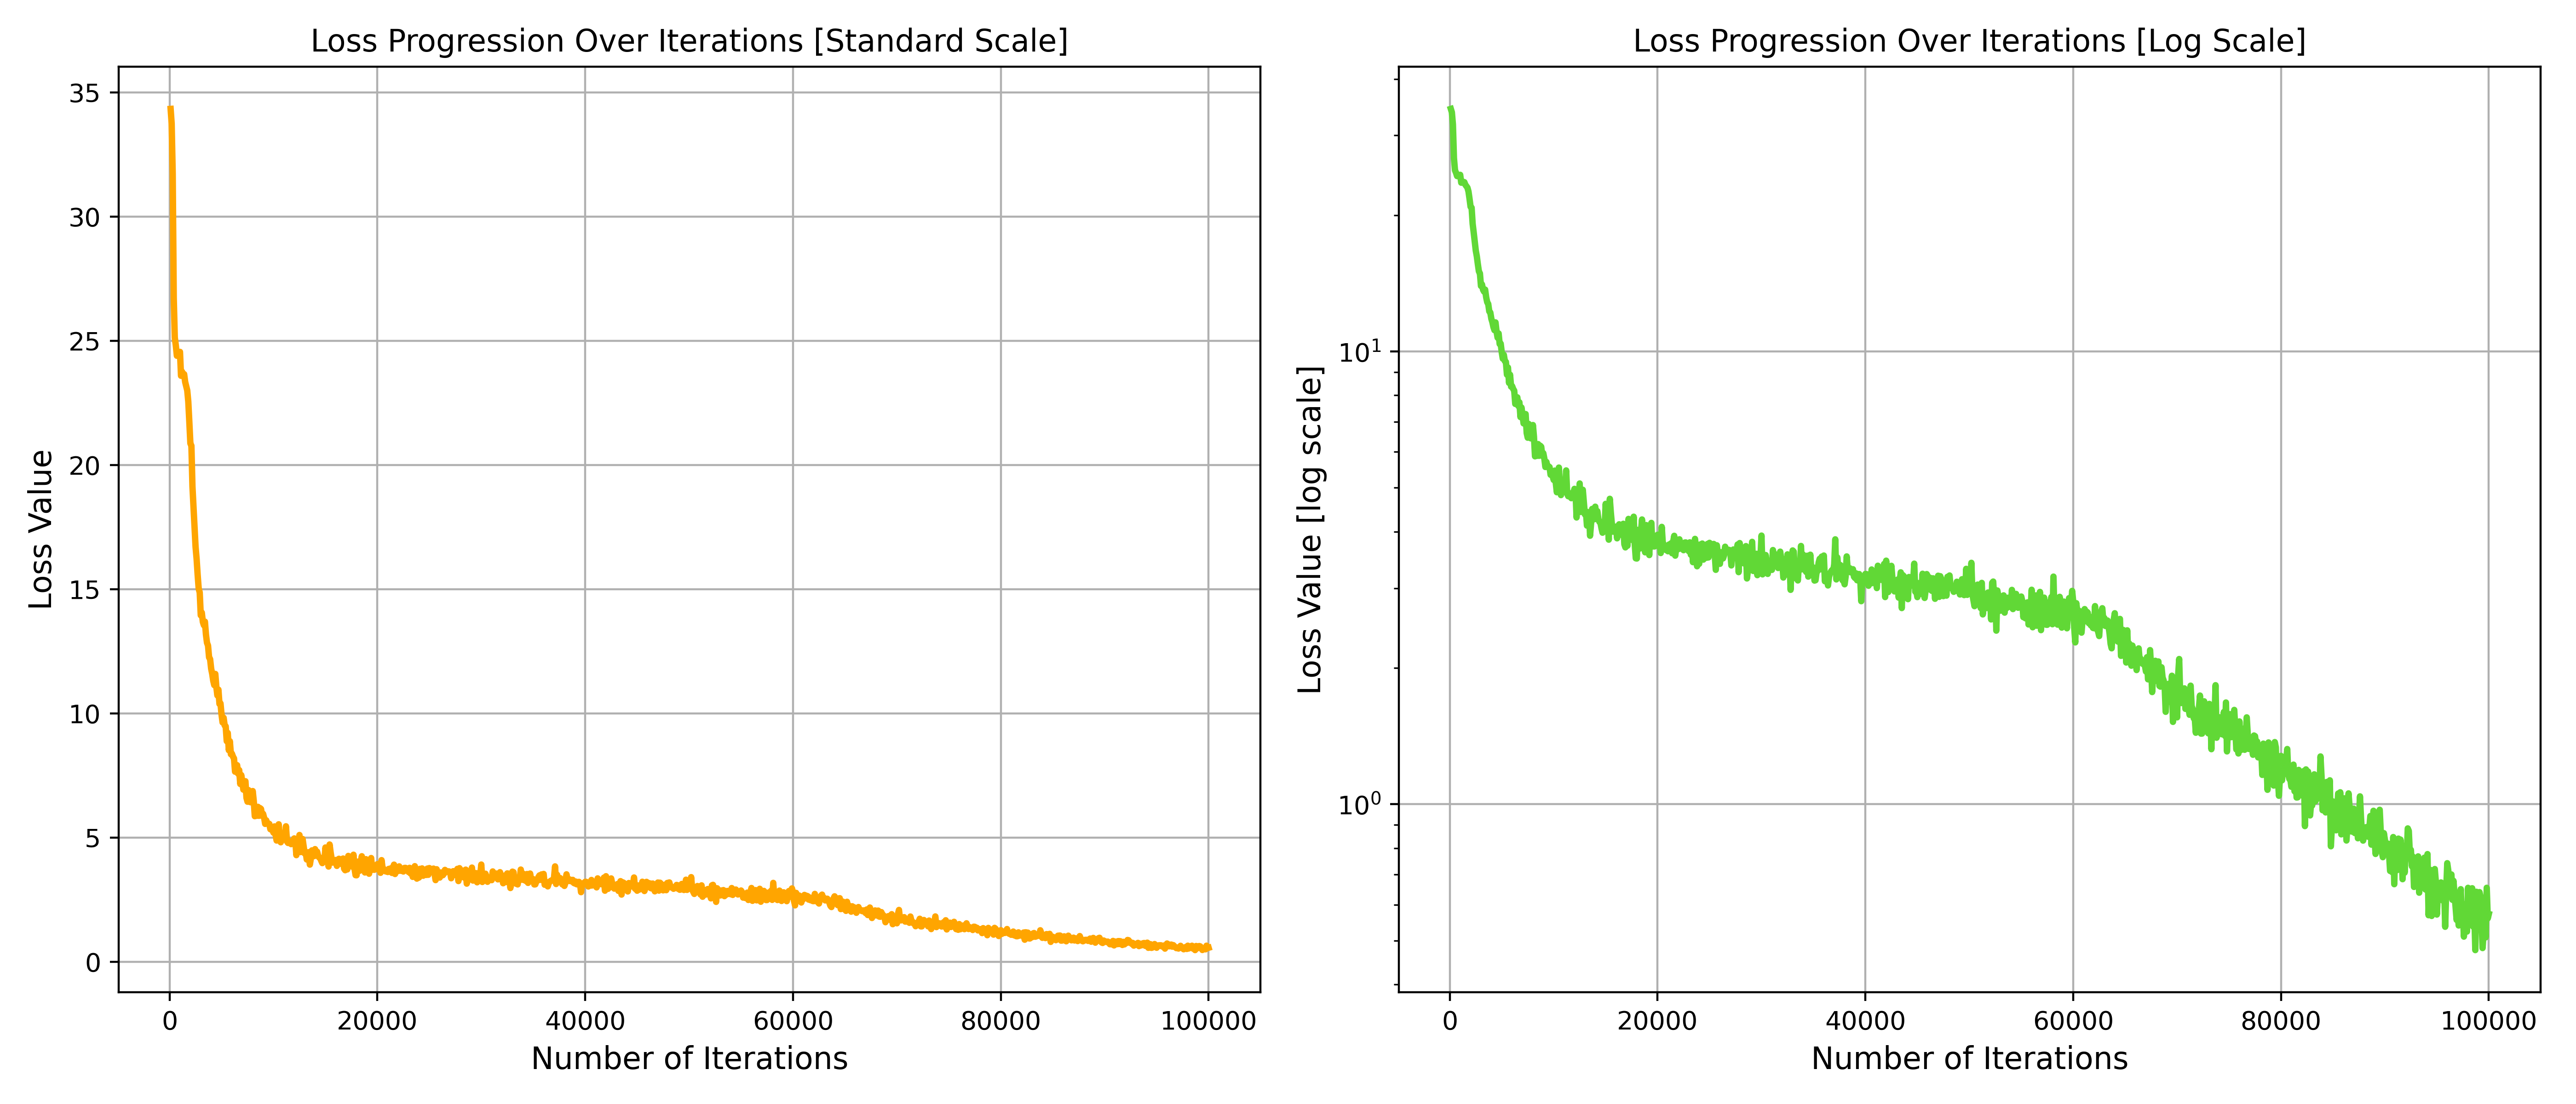
\includegraphics[width=1\linewidth]{LateX//figs/loss_total_mse_progression_comparison.png}
    \caption{Total Loss Progression Using MSE as the Loss Function}
    \label{fig:mse-loss-progression}
\end{figure}

Focusing on specific losses for the pose and heading angle, the following behavior was observed:

\begin{figure}[H]
    \centering
    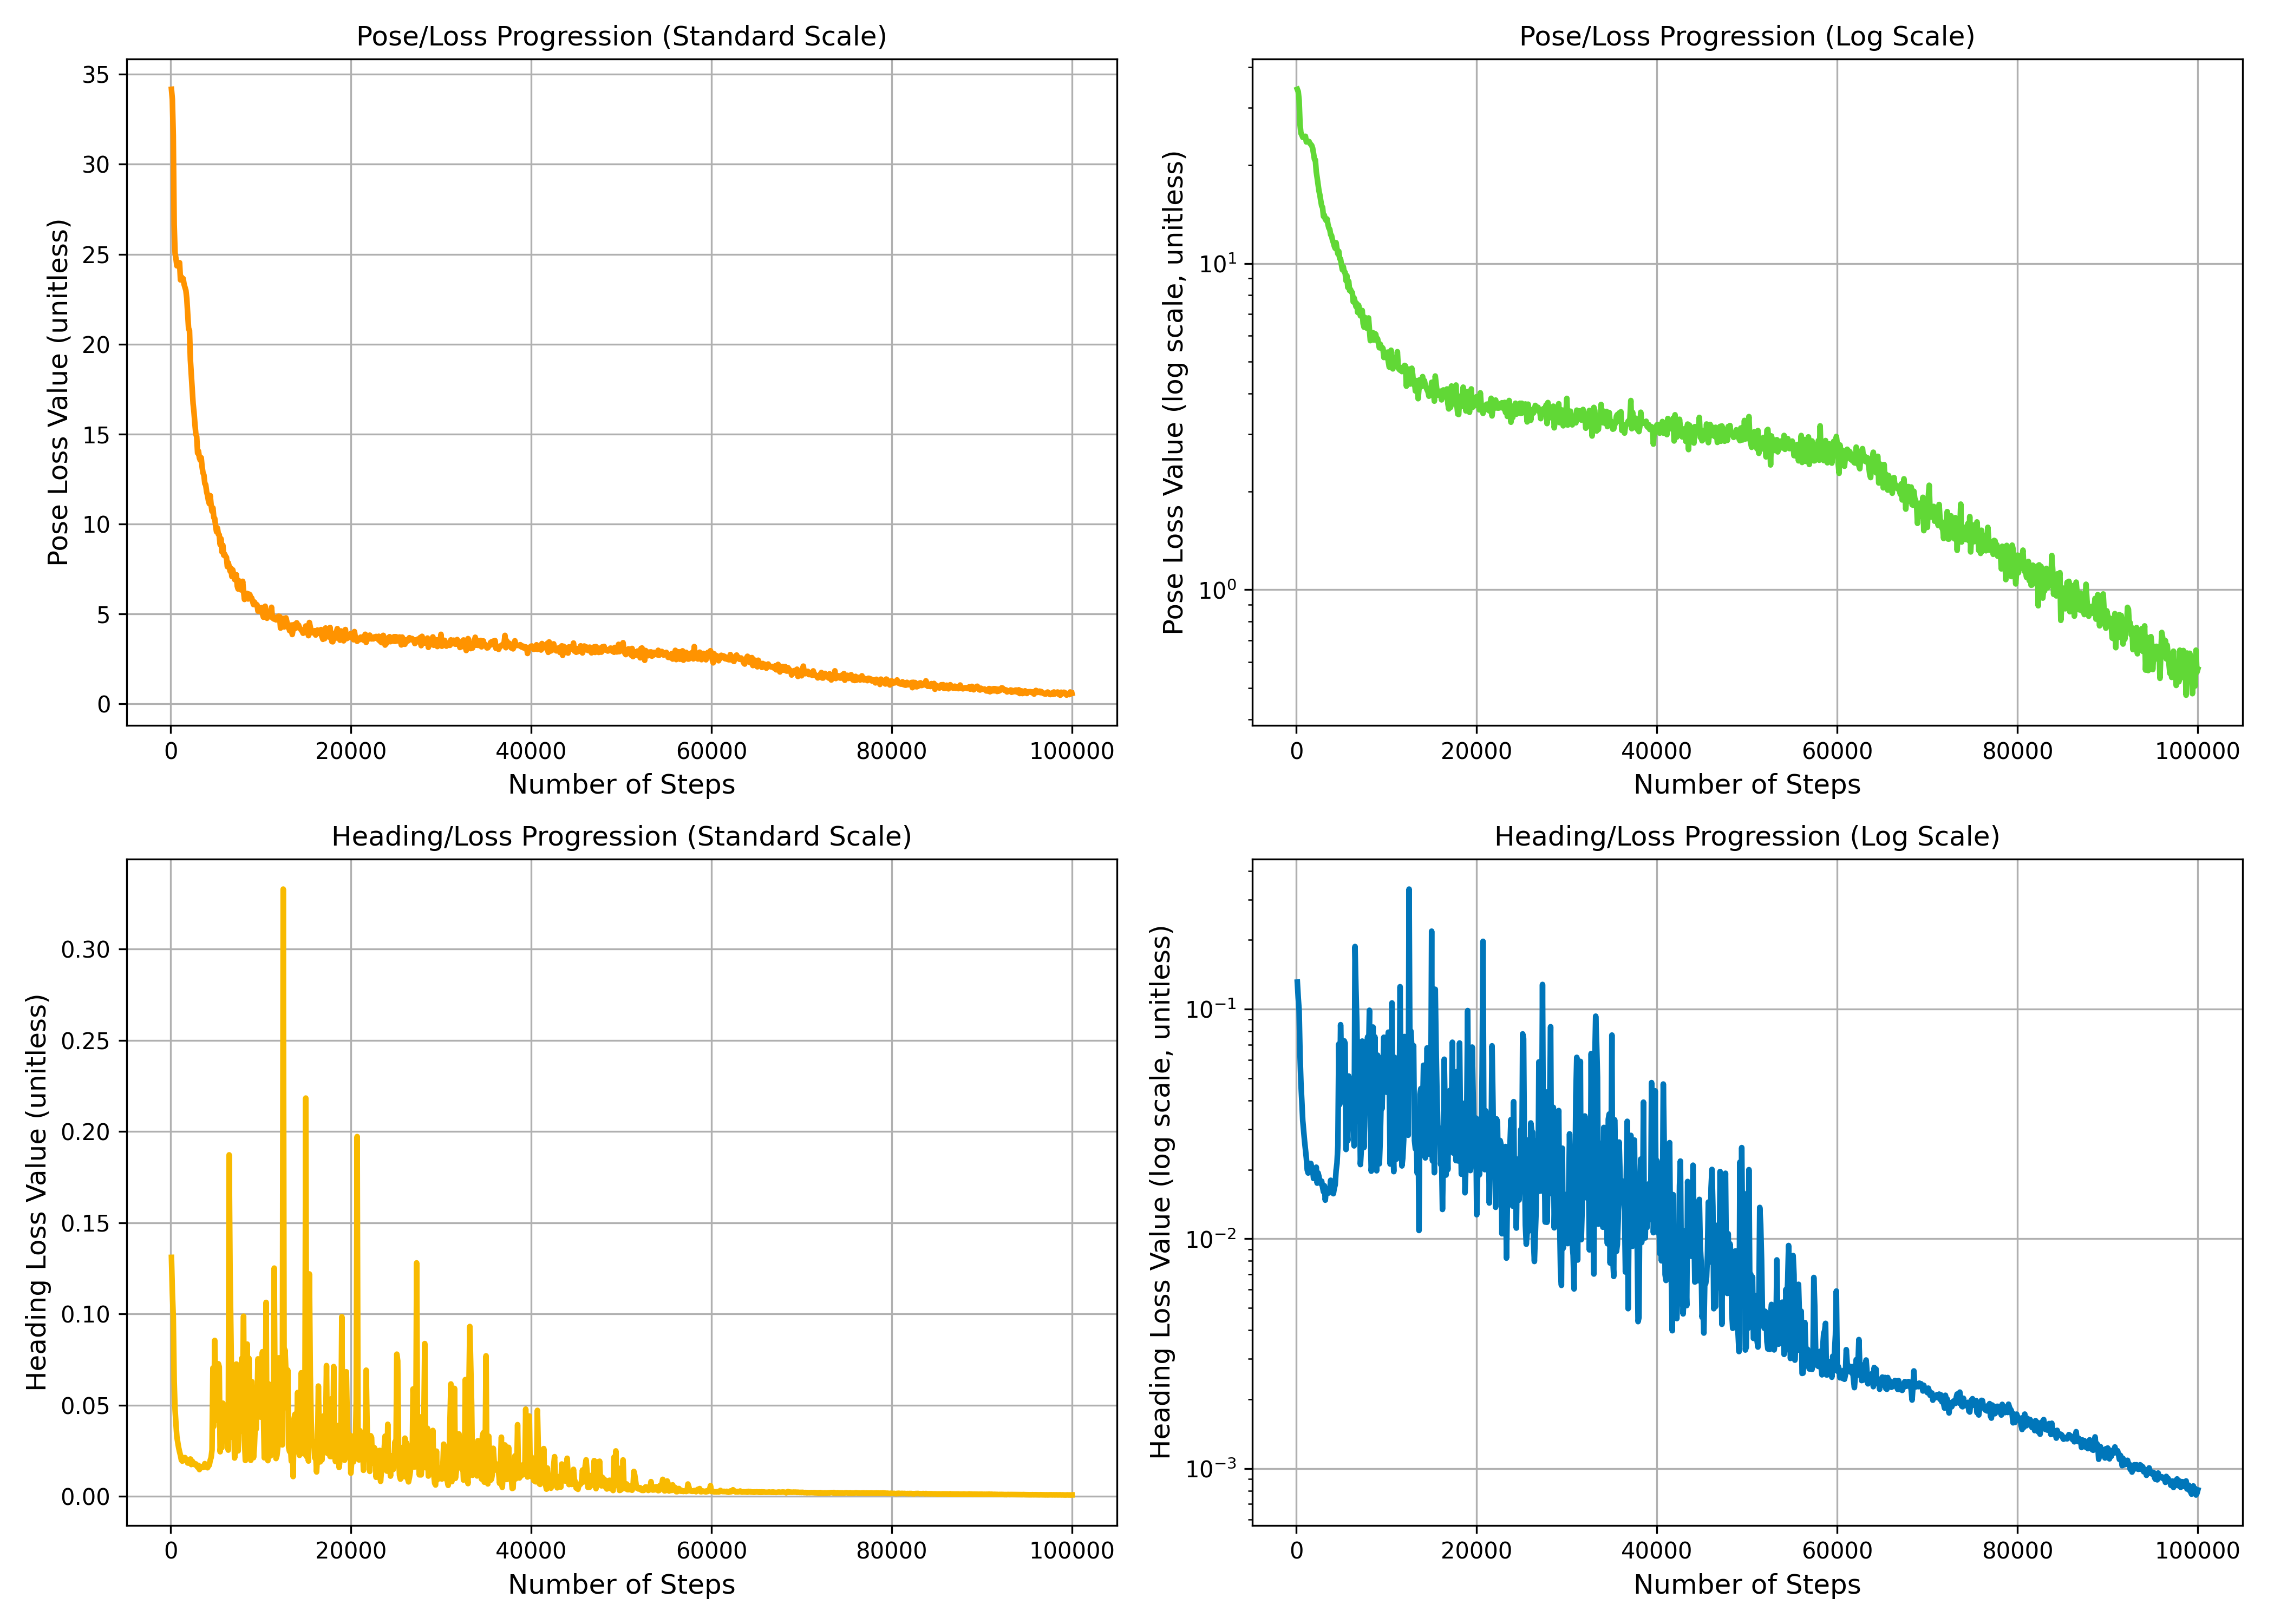
\includegraphics[width=1\linewidth]{LateX//figs/mse_pose_heading_loss_comparison.png}
    \caption{Pose and Heading Loss Comparison During Training}
    \label{fig:pose-heading-loss}
\end{figure}

The model's behavior during evaluation aligned with expectations, and the training evaluations yielded the following results:

\begin{figure}[H]
    \centering
    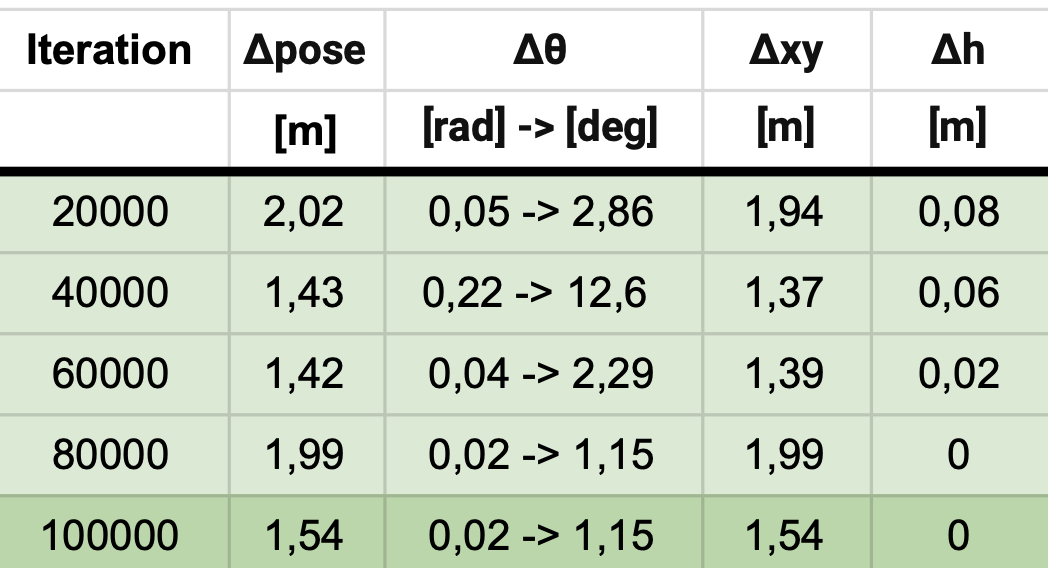
\includegraphics[width=0.75\linewidth]{LateX//figs/tabella_iteration1.png}
    \caption{Evaluation Results for Initial Iterations (Table to be updated)}
    \label{fig:evaluation-results}
\end{figure}

\textbf{Comment on Results:} Despite the loss functions decreasing and reaching very low values, indicating potential generalization and effective learning, the evaluation process reveals that the results are still not optimal or acceptable. The positional error exceeds one meter, which is not sufficient for HD map alignment applications, as discussed in Chapter 1. Consequently, we decided to test alternative loss functions to determine if a different loss could improve the model’s learning process.

\subsection*{L1 Loss}
Using the L1 loss, defined similarly to the previous setup, the total loss was supplemented by two specific auxiliary losses. The results with L1 loss are consistent with previous observations. As shown in the results table below, the behavior was similar to the prior experiments, although with slightly lower values.

Since the specific loss graphs did not reveal significant differences, only the results table is provided for this experiment.

\begin{figure}[H]
    \centering
    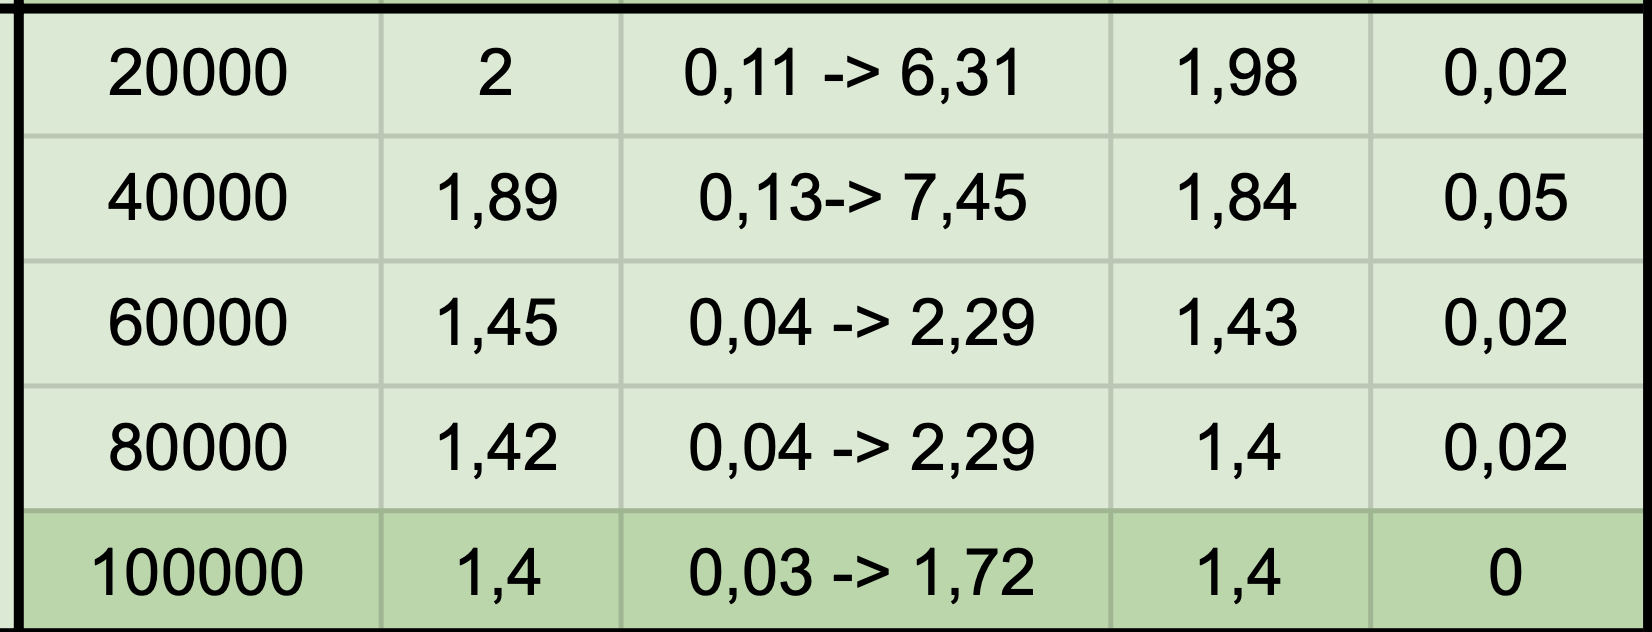
\includegraphics[width=0.5\linewidth]{LateX//figs/tabella_l1.png}
    \caption{Evaluation Results for L1 Loss (Table to be updated)}
    \label{fig:l1-loss-results}
\end{figure}

\subsection*{Smooth L1 Loss}
In this experiment, the Smooth L1 loss, similar to L1 but less sensitive to outliers, was used. The training results remained consistent with expectations, but this time some interesting differences emerged, as the results showed slight improvements over previous attempts. Both loss graphs and the evaluation table are provided below to illustrate this behavior.

\begin{figure}[H]
    \centering
    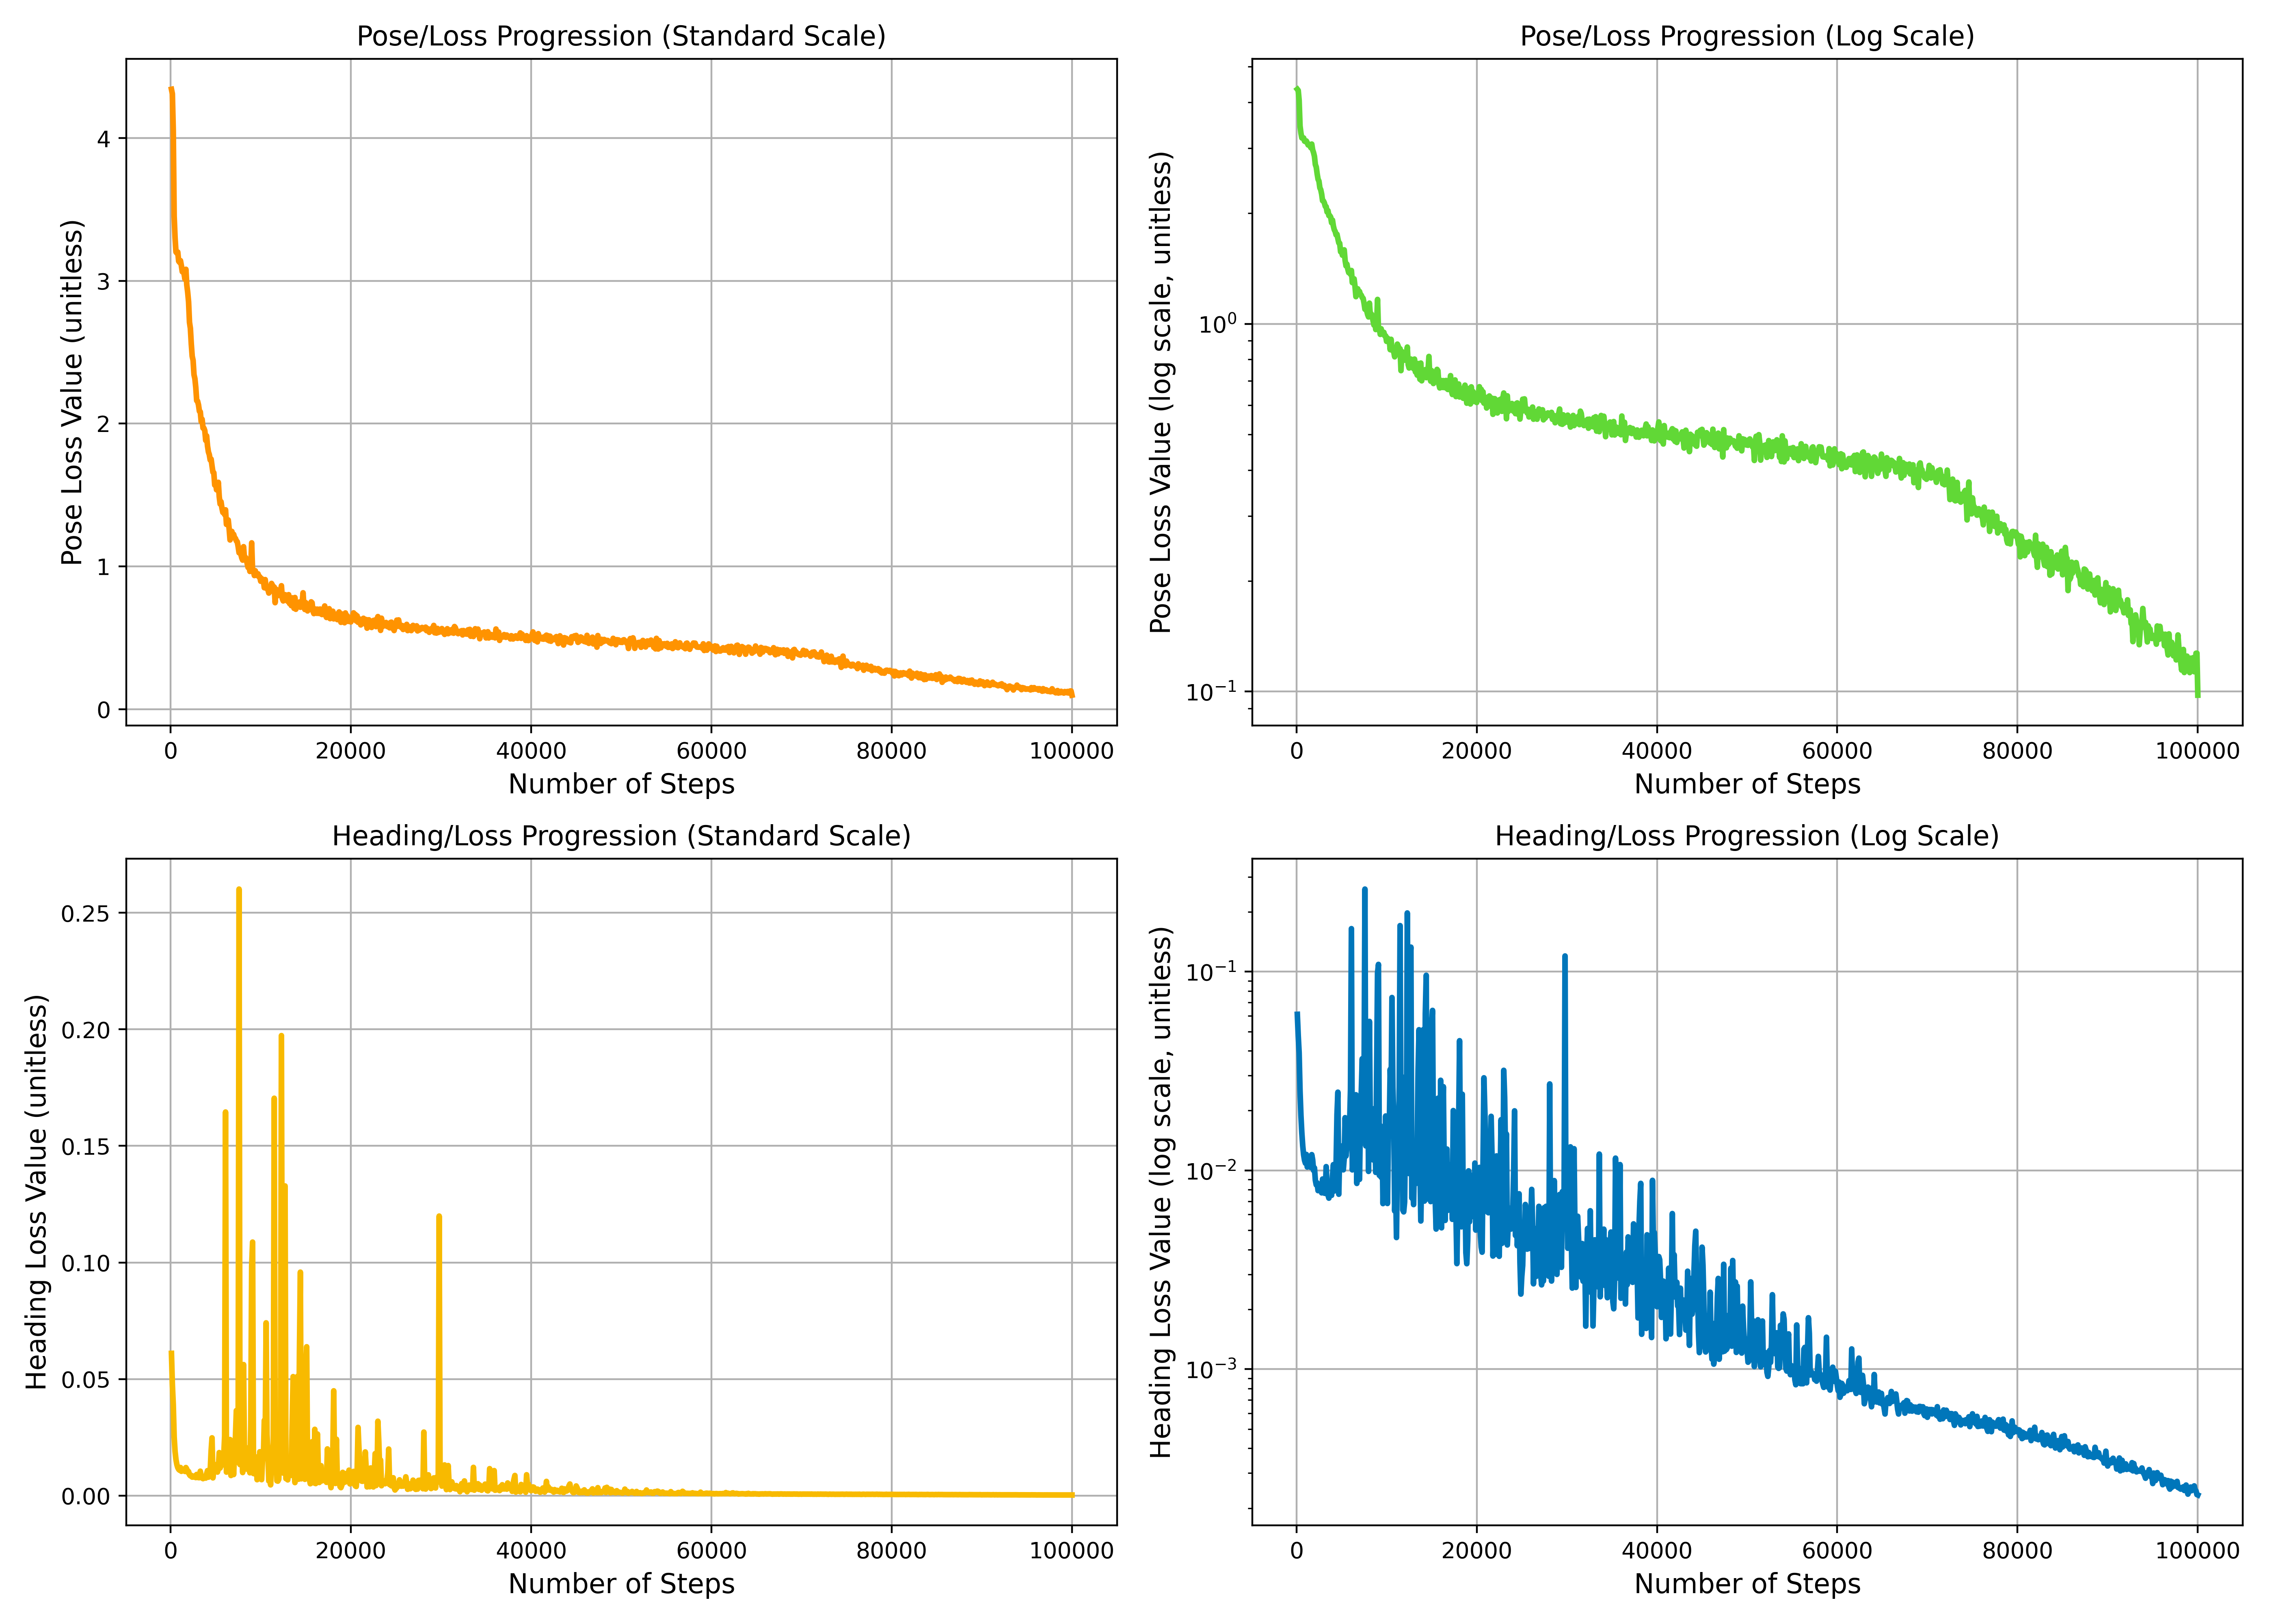
\includegraphics[width=0.75\linewidth]{LateX//figs/l1s_pose_heading_loss_comparison.png}
    \caption{Pose and Heading Loss Comparison Using Smooth L1 Loss}
    \label{fig:smooth-l1-pose-heading-loss}
\end{figure}

\begin{figure}[H]
    \centering
    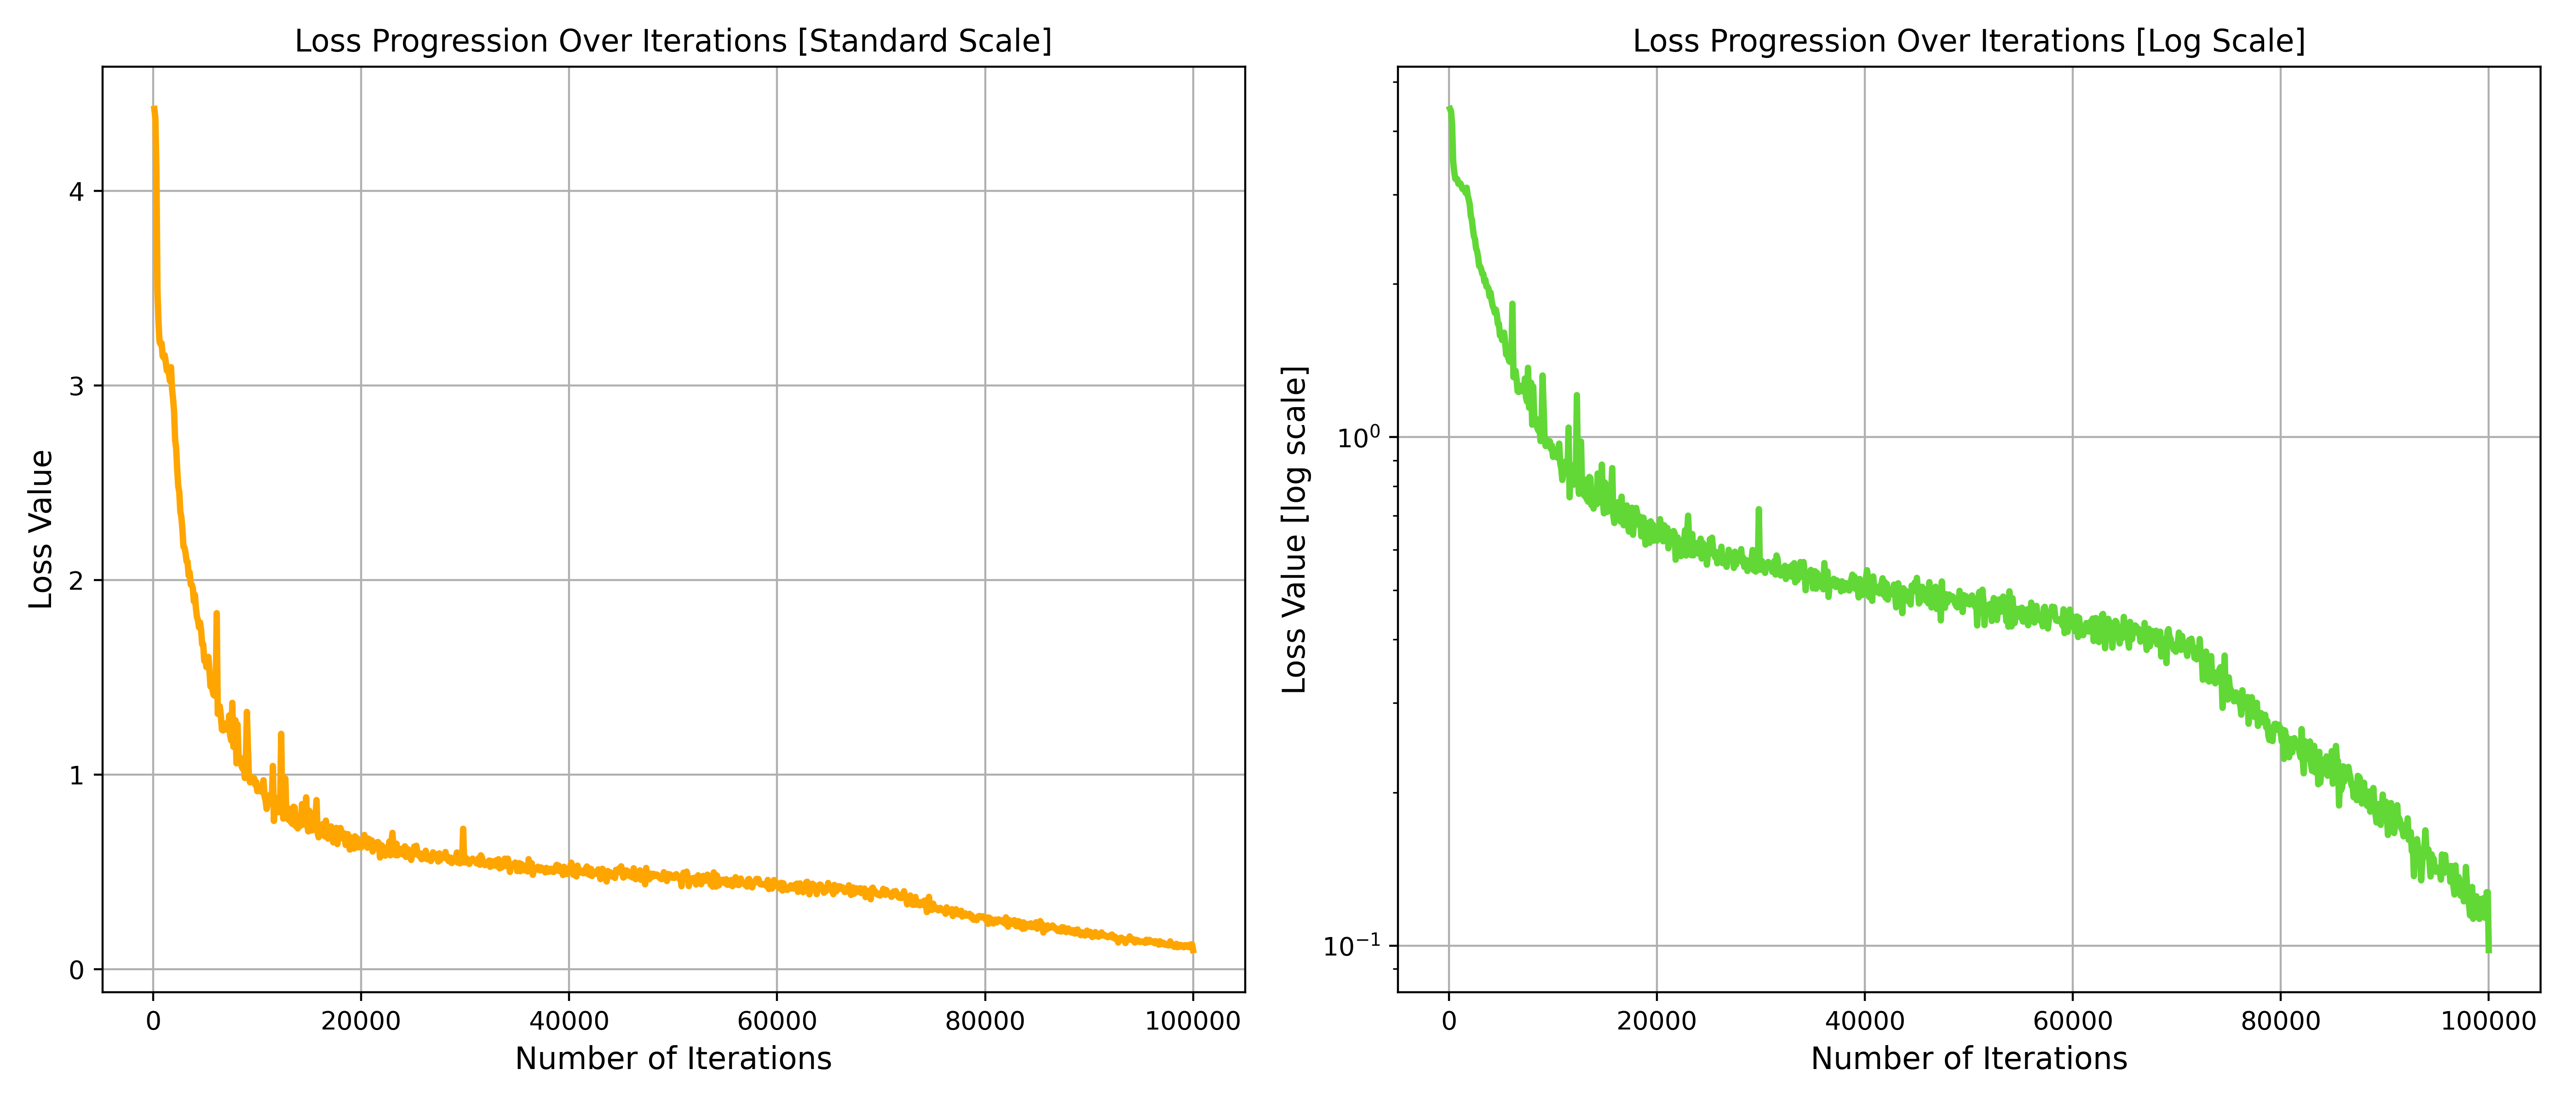
\includegraphics[width=0.75\linewidth]{LateX//figs/loss_total_l1s_progression_comparison.png}
    \caption{Total Loss Progression Using Smooth L1 Loss}
    \label{fig:smooth-l1-total-loss}
\end{figure}

A summary of the evaluation results during training is shown below:

\begin{figure}[H]
    \centering
    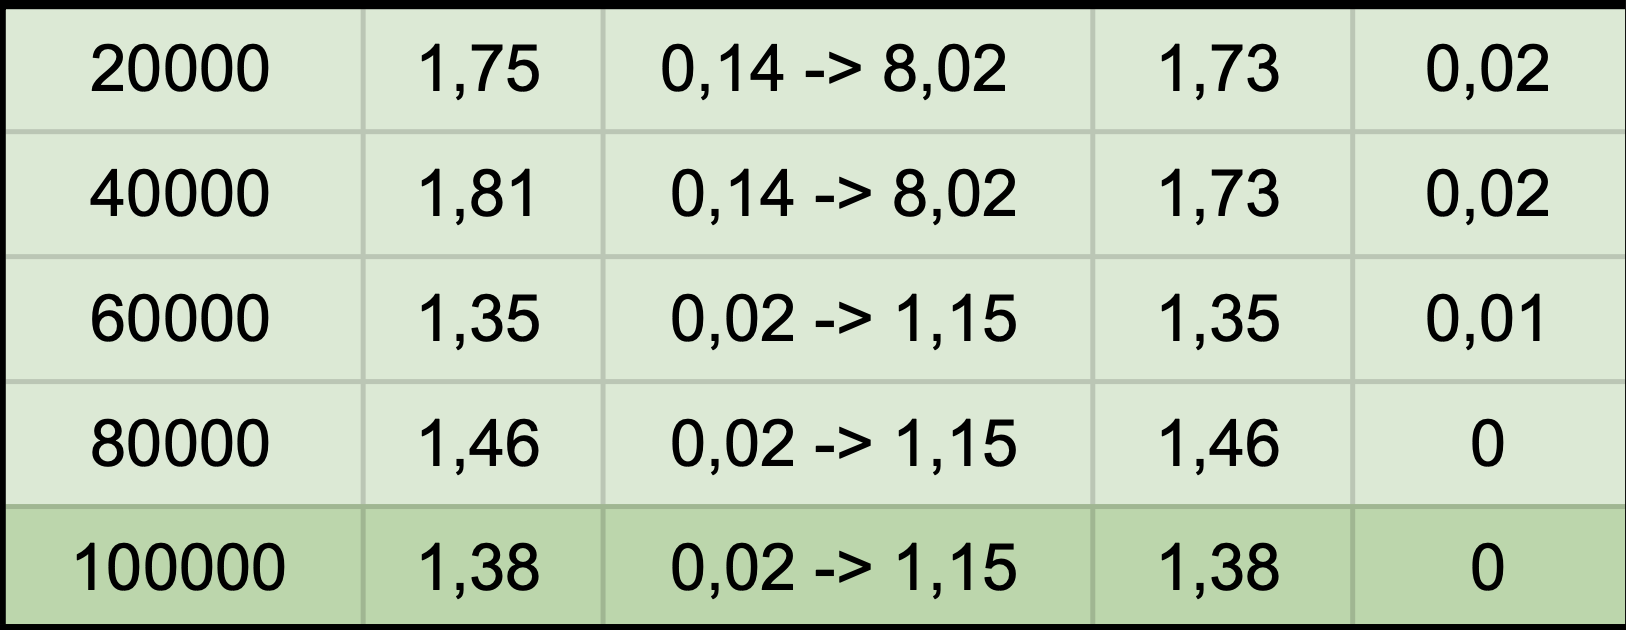
\includegraphics[width=0.5\linewidth]{Screenshot 2024-11-14 at 11.50.25.png}
    \caption{Summary of Evaluation Results for Smooth L1 Loss (Table to be updated)}
    \label{fig:smooth-l1-evaluation}
\end{figure}

As indicated in the table, the Smooth L1 loss yielded the best results. This outcome aligns with the characteristics of Smooth L1 loss, which merges the benefits of L1 and L2 losses. It reduces sensitivity to outliers more effectively than MSE loss, while balancing convergence speed and stability. This makes it particularly suitable for regression tasks involving spatial transformations.

To ensure the network’s predictions are on a similar scale, facilitating learning, the heading angle (initially in radians) was converted to degrees. This adjustment corrected a scale imbalance, as angle values in radians were significantly smaller than the translation values. The same experiments were repeated after this adjustment, using the same loss functions, with results shown below.

\begin{figure}[H]
    \centering
    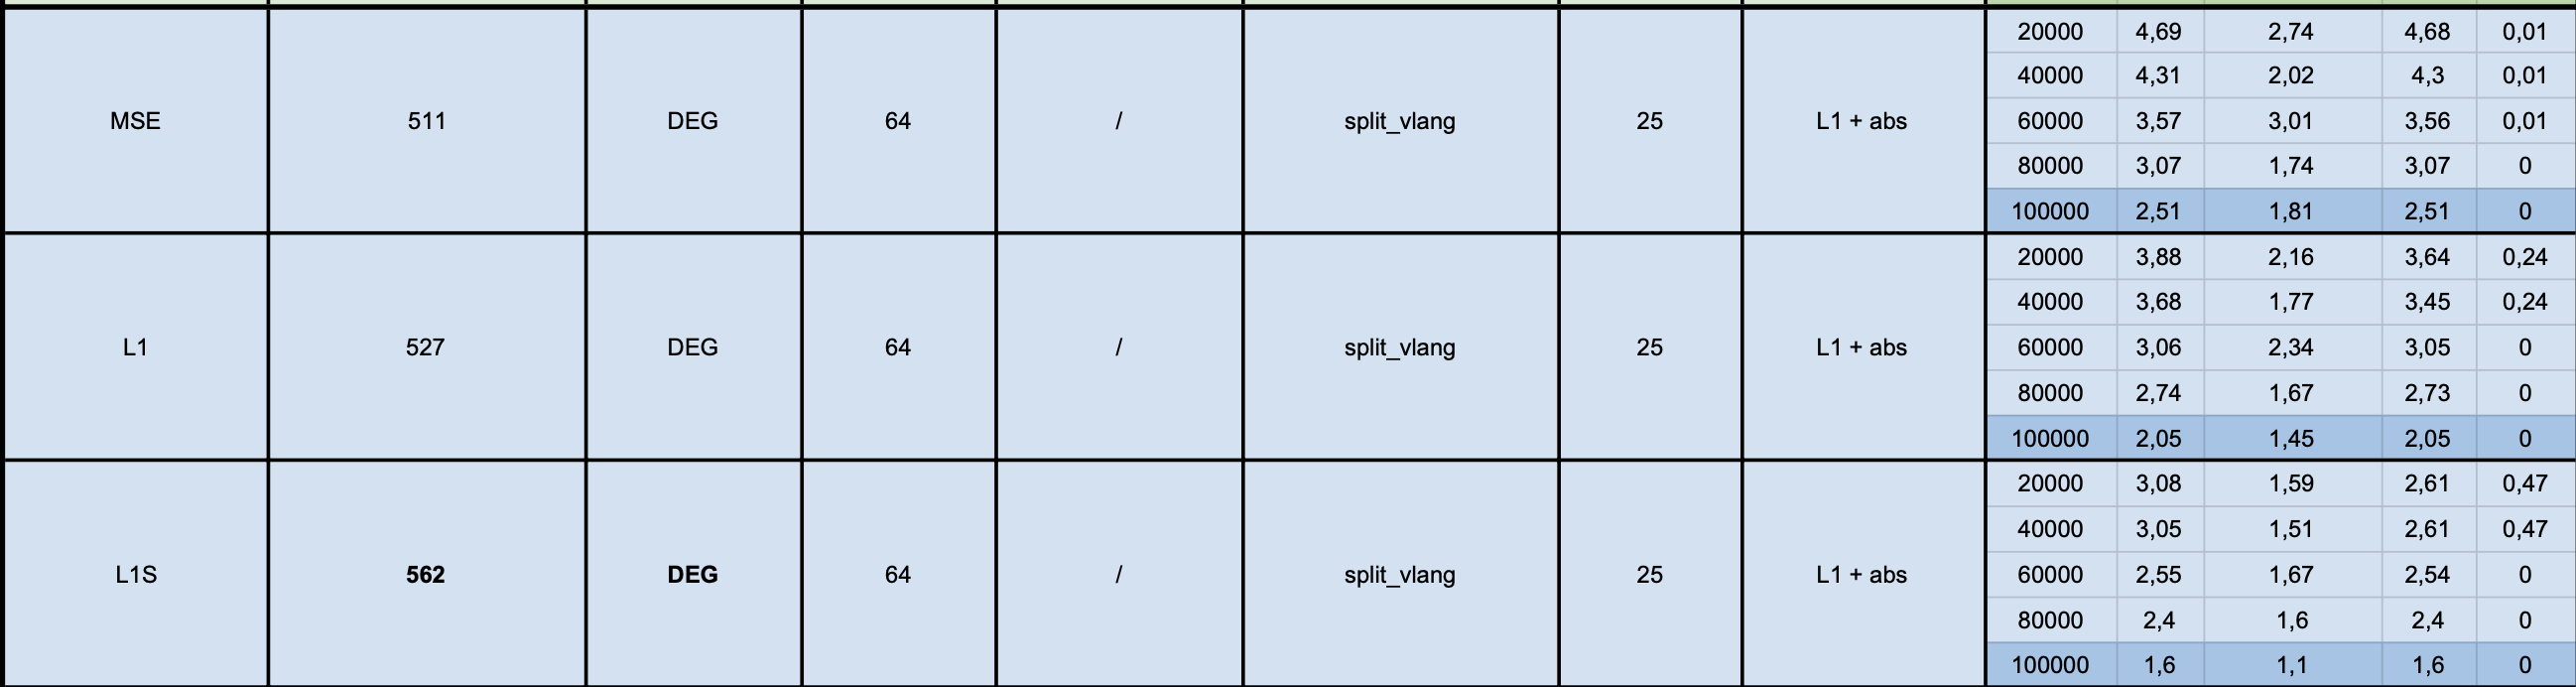
\includegraphics[width=1\linewidth]{Screenshot 2024-11-14 at 11.52.27.png}
    \caption{Evaluation Results with Heading Angle in Degrees (Table to be updated)}
    \label{fig:degree-evaluation-results}
\end{figure}

As expected, scaling the heading angle to degrees improved the results, reducing errors and bringing predicted values closer to desired outcomes. Once again, the Smooth L1 loss provided the best generalization performance.

These findings highlight the importance of consistent value scales across predicted parameters and the effectiveness of Smooth L1 loss in training models for spatial transformation estimation.

Given these findings, when the full dataset was utilized by merging all sequences from the three streets, only the best-performing model from the preliminary analysis (using Smooth L1 loss) was tested. The results are shown and discussed below.

\textbf{Full Dataset Results:} The graphs below show improvements in angle prediction, aided by the increased data volume, Smooth L1 loss, and the angle conversion to degrees. However, the main issue remains with translation error. Despite improvements, further refinement or the use of a more precise optimization method is needed to achieve accurate HD map alignment. This model version could potentially assist in challenging scenarios but does not fully solve the alignment problem.

\subsection{Inference}
Inference was also tested on an unseen sequence that was not part of the training dataset. This sequence contained long stretches of straight road, with few distinctive textures or reference points. During inference, it appeared that the network attempted to minimize the distance but from the wrong boundary, creating good alignment for the angle but misaligning the translation by an entire lane width. An example of this behavior is shown below:
